\section{Results}
\label{sec:results}

\begin{figure}
\centering
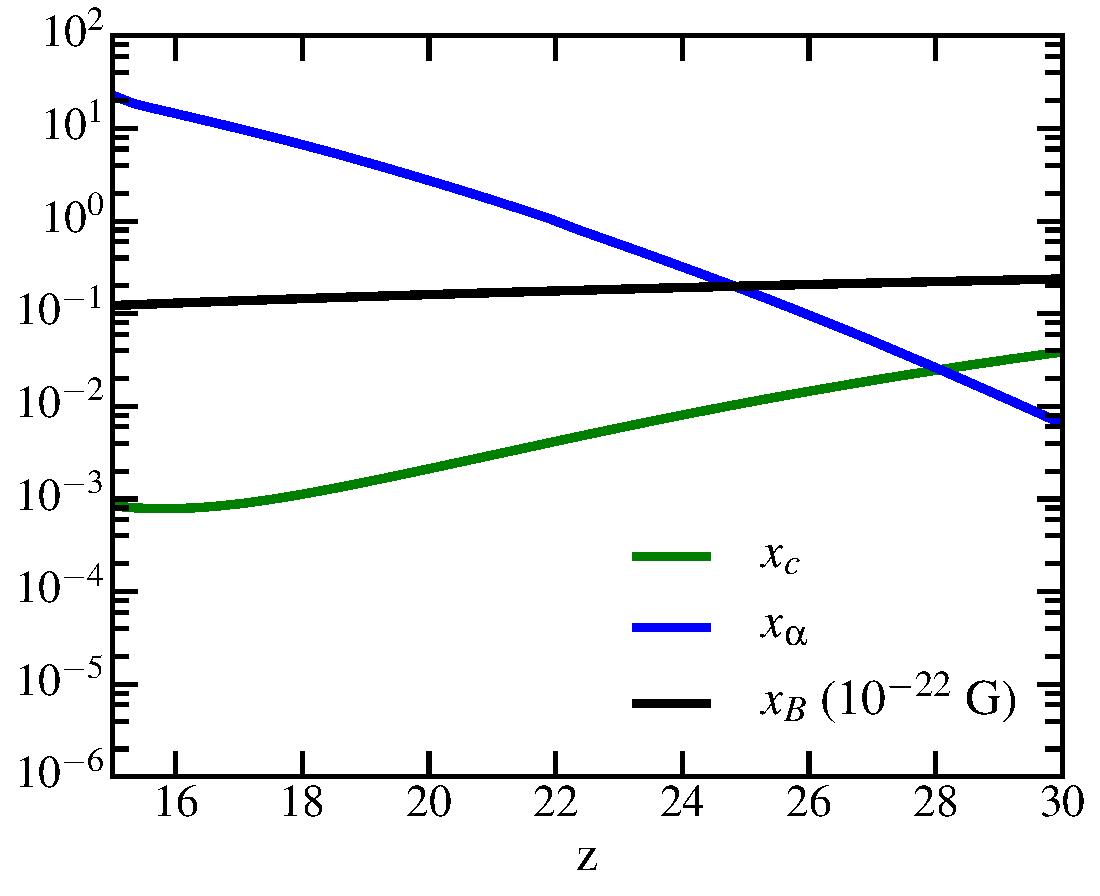
\includegraphics[width=.35\textwidth,keepaspectratio=true]{xs.pdf}
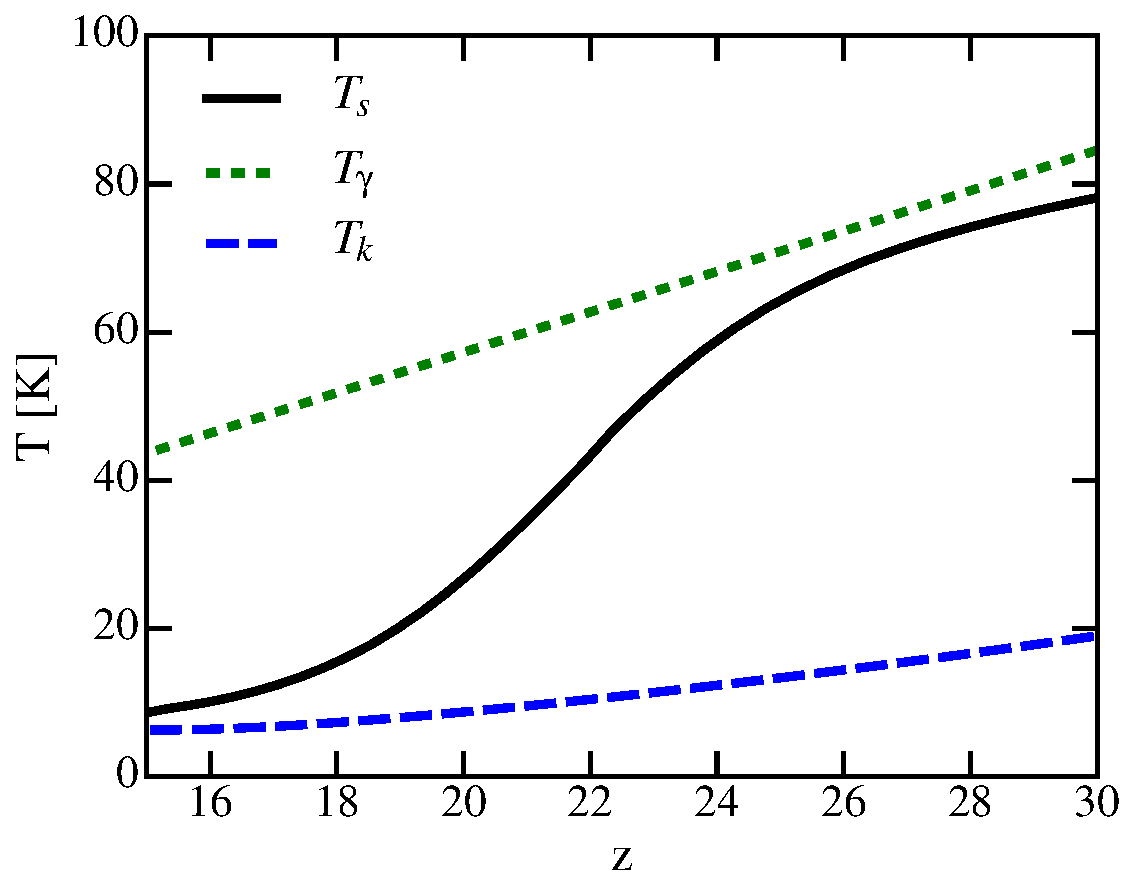
\includegraphics[width=.35\textwidth,keepaspectratio=true]{Ts.pdf}
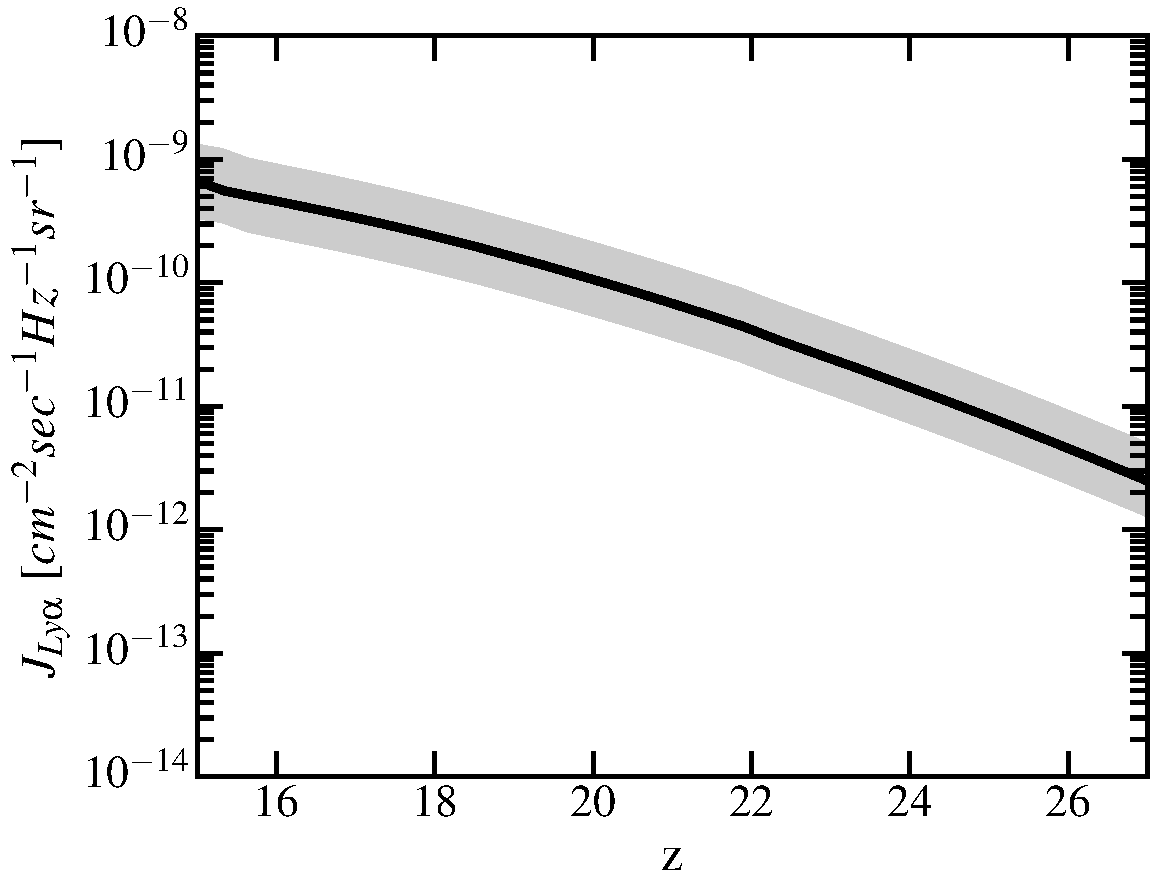
\includegraphics[width=.35\textwidth,keepaspectratio=true]{Jlya.pdf}
\caption{Inputs for sensitivity calculation: Lyman-$\alpha$ flux model computed for standard cosmology using \texttt{21cmfast}, and the relevant spin- and kinetic- temperature models. \label{fig:cosmo}}
\end{figure}
We now proceede to numerically evaluate the sensitivity of 21--cm tomography to detecting magnetic fields during the pre-reionization epoch, using the formalism we developed in previous two Sections. For this purpose, we only focus on one type of experimental setup---an array of dipole antennas arranged in a compact grid, such as implemented in HERA, for example. The motivation behind this choice is that such configuration is known to maximize sensitivity to recovering statistics of the cosmological 21--cm signal \cite{2009PhRvD..79h3530T,2015AAS...22532803D} in general. We consider an array with a collecting area of $(\Delta L\text{ km})^2$, where $\Delta L$ is taken to be maximal baseline separation.

The observation time $t_1$ (appearing in the expression for the noise in Eq.~(\ref{eq:Pnoise_K})) for a total duration of the survey  $t_\text{obs}$ is a function of the type of the experiment.  For a radio dish with a beam of a solid angle $\Omega_\text{beam}=\lambda^2/A_e$ which is much smaller than the size $\Omega_\text{survey}$ of the survey, the telescope scans the sky one beamwidth at a time. In that case, $t_1$ is the total time spent observing one $(u,v)$ element,$t_1=t_\text{obs}\Omega_\text{survey}/\Omega_\text{beam}$. However, in the case of an array of dipoles we are considering here, the beam is greater than (or equal to) the survey size, and $t_1=t_\text{obs}$. We do not explicitly account for the fact that any given patch of the sky is only visible for a part of the day from a given location; therefore, $t_\text{obs}$ we substitute in the noise calculation is shorter than the wall--clock duration of the survey by a factor of a few. To derive numerical results, we assume $\Omega_\text{survey}=1$sr, and the wall--clock survey duration of about 2 years (corresponding to $t_\text{obs}=1$ year). 

For the sky temperature that enters the noise power spectrum in \eq{\ref{eq:Pnoise_K}}, we assume a simple model of Galactic synchrotron emission from Ref.~\cite{2008PhRvD..78b3529M}, 
\beq
T_\text{sky}  = 60\left(\frac{21}{100} (1+z)\right)^{2.55}\text{   [K]}.
\label{eq:tsys}
\eeq

Other ingredients entering our sensitivity calculation are the mean Lyman--$\alpha$ flux $J_{\text{Ly}\alpha}(z)$, the spin $T_s$ and kinetic $T_k$ temperatures of the IGM, and the CMB temperature $T_\gamma$, all functions of redshift. These are all obtained using \texttt{21CMFAST} code \cite{2011MNRAS.411..955M}. As input to \texttt{21CMFAST}, we used cosmological parameters consistent with Planck cosmology \cite{2015arXiv150201589P}, while keeping other input parameters at their default values, with the exception of the star formation efficiency, \verb|F_STAR|. For our fiducial calculation, we choose the value of \verb|F_STAR|=$0.0075$, corresponding to the solid lines in Figure \ref{fig:cosmo}. The top panel shows quantities (discussed in Paper I) that parametrize the rates of depolarization of the ground state by optical pumping, atomic collisions, and magnetic precession. The middle panel shows the relevant gas and CMB temperatures. The bottom panel shows $J_{\text{Ly}\alpha}(z)$, where the solid line, as before, corresponds to the fiducial choice of parameters, while the gray band of ``uncertainty'' around this curve corresponds to \verb|F_STAR|$=0.0025$ and \verb|F_STAR|$=0.01875$. The fiducial choise produces a match of the flux to the models in Ref.~\cite{2012ApJ...746..125H} at $z=15$, while the gray band (the ``extreme'' parameter values) are chosen to roughly capture the level of uncertainty in the flux modeling at high redshifts (given the lack of direct observation at high $z$). We use these extreme models (corresponding to the bounds of the gray band in this Figure) to test sensitivity of our key results to the uncertainty in the evolution of the Lyman--$\alpha$ flux and other input parameters (note that we do not plot corresponding ``uncertainty bands'' on the other two panels, simply to avoid clutter; but we use them consistently in our sensitivity calculation, as discussed below). We assume that the redshift range covered by the survey is $z\in[15,35]$. %more on z range and on 21cmfast


\begin{figure}
\centering
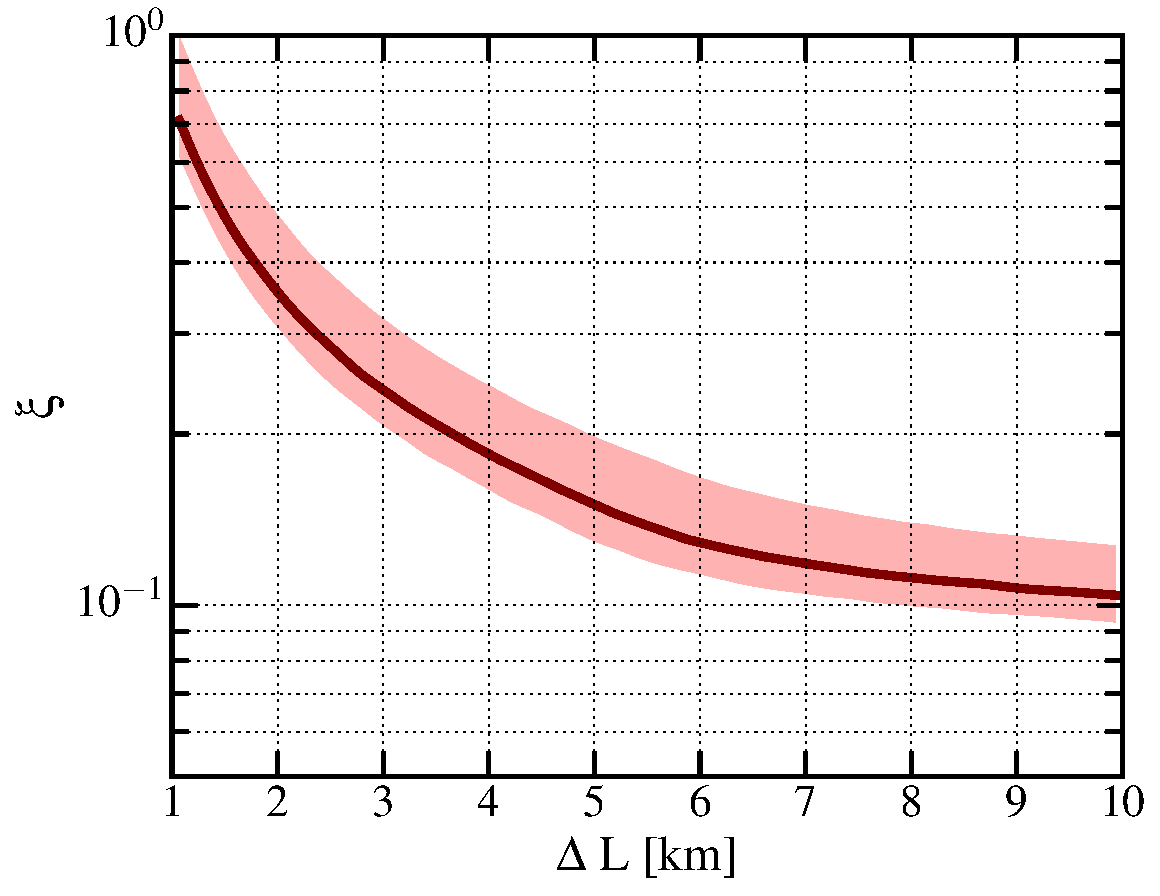
\includegraphics[width=.35\textwidth,keepaspectratio=true]{xi_vs_deltas.pdf}
\caption{Sensitivity to detecting magnetic field in the saturated regime (upper panel), as a function of maximum array baseline (or, equivalently, of the total collecting area, ($\Delta L)^2$), assuming a survey size of 1 sr and survey duration of 2 years. The light--colored band around the solid line corresponds to the Lyman-$\alpha$ model flux uncertainty, represented with a gray band in Figure \ref{fig:cosmo}.\label{fig:xi_vs_deltas}}
\end{figure}
\begin{figure}
\centering
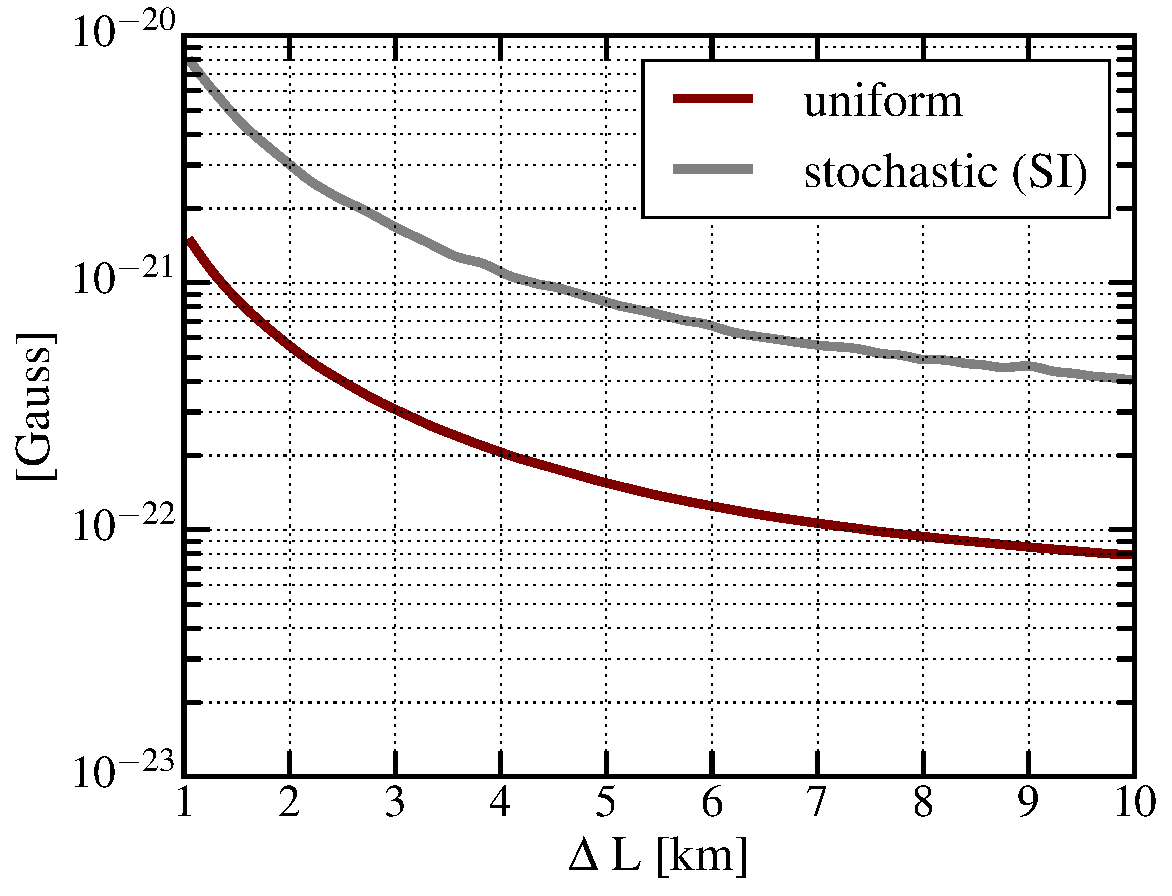
\includegraphics[width=.35\textwidth,keepaspectratio=true]{B_vs_deltas.pdf}
\caption{Sensitivity to detecting a uniform and stochastic magnetic field (stochastic field is assumed to have a scale--invariant (SI) power spectrum, and shown is the root--mean--squared per $\log K$, that is $A_0/\pi$.), as a function of maximum array baseline, assuming a survey size of 1 sr, and for survey duration of 2 years.\label{fig:B_vs_deltas}}
\end{figure}
Figures \ref{fig:xi_vs_deltas} and \ref{fig:B_vs_deltas} show the key results: the sensitivity of the tomographic survey as a function of the maximum baseline $\Delta L$ (where different baselines may correspond to different stages of a single experiment). Figure \ref{fig:xi_vs_deltas} shows $1\sigma$ sensitivity to measuring parameter $\xi$ of \eq{\ref{eq:saturated_P}}, which quantifies the distinction between the case of no magnetic field and the case where the field is strong and the signal is in a saturated regime. The value of this parameter is, by definition, bound between 0 and 1, where 0 represents the case of no magnetic field, and 1 represents the saturated case. In this Figure, the solid line represents fiducial calculation, while the light--colored band around it corresponds to the uncertainty band of the inputs shown in Figure \ref{fig:cosmo}. The fiducial result implies that an array with one kilometer squared of collecting area can achieve $1\sigma$ detection threshold, which can be interpreted as follows. If a survey were to measure $\xi\ne 0$, that would be a $1\sigma$ detection of a lower bound on a uniform magnetic field in the entire survey volume. The value of the lower bound as a function of redshift would correspond to the saturation ceiling at that redshift, which can be roughly evaluated from the condition that the depolarization rates through standard channels equal the rate of depolarization via magnetic precession, $x_B = 1+x_{\alpha ,(2)} +x_{c,(2)}$. The ceiling is depicted with a dashed line in Figure \ref{fig:Bsat}, and it corresponds to $|\vec B|\sim 2\times 10^{-21}$ Gauss (comoving) at $z=20$, for example.  On the other hand, if a survey were to report a null result, it would rule out such magnetic field, at the same confidence level. In that case, an upper bound on the strength of the magnetic field components in the plane of the sky can be computed, as discussed in the following. 

Figure \ref{fig:B_vs_deltas} is obtained by evaluating the expressions of Eqs.~(\ref{eq:fisher_patch}) and (\ref{eq:snr_ints}), and it shows a $1\sigma$ upper bound that can be placed on the value of the magnetic field, in case of no detection. The result is shown for both the uniform field (lower solid red line), and for the amplitude of a stochastic field (upper gray line) with the scale--independent power spectrum. While the numerical calculation assumed that the brightness temperature is a linear function of the field strength, this assumption is not guaranteed to hold---it breaks down in the saturation limit, as discussed above and in \S\ref{sec:method}. So, this Figure is only valid if $\xi=0$.

In order to understand how the projected constraints (sensitivities) presented in Figure \ref{fig:B_vs_deltas} compare to the saturation ceiling at the redshifts we consider, Figure \ref{sigmaB0_vs_z.pdf} shows a comparison between the saturation ceiling and the values of the $z$--dependent integrands of \eq{\ref{eq:fisher_patch}} (plotted for several array sizes). We can now see that the sensitivity to the uniform field corresponding to all array sizes in consideration is below the saturation regime for the redshifts where most of the SNR comes from: $z\sim$20--21 (the minima of these curves). This gives us confidence that the results for the uniform field in Figure \ref{fig:B_vs_deltas} are indeed valid, and the linear theory holds in the given regime. For the SI case, however, it is likely that a factor of a few larger array sizes are needed to achieve sensitivity that is below the saturation limit at relevant redshifts. It is also important to note here that the calculation of the saturation ceiling presented in this Figure is quite conservative, where in reality  linear theory should hold well until the field reaches a value that is a few times above this level.
\begin{figure}
\centering
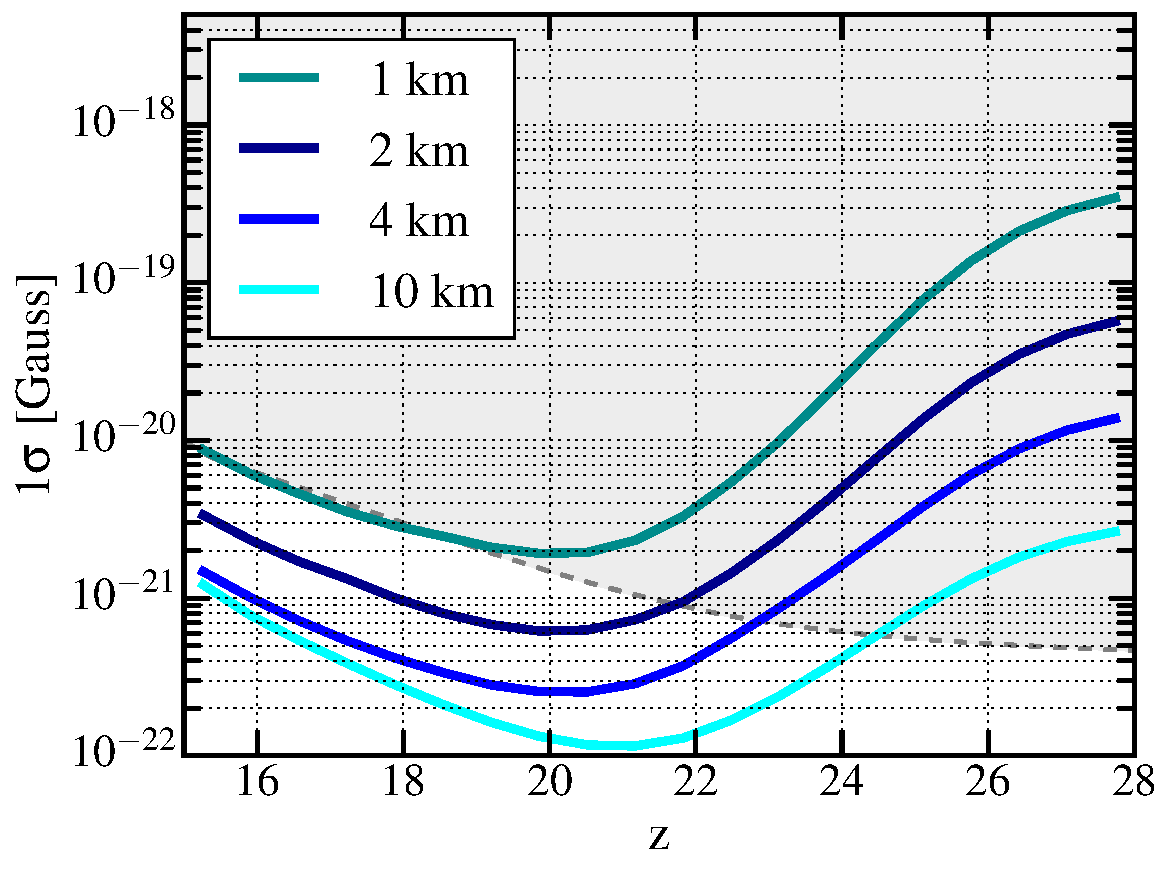
\includegraphics[width=.35\textwidth,keepaspectratio=true]{sigmaB0_vs_z.pdf}
\caption{Saturation regime is shown as a shaded gray area above the dashed curve. Integrand of \eq{\ref{eq:fisher_patch}} (inverse sqare root of it) is shown as a function of redshift, for several maximum---baseline lengths.  When the colored curves are below the saturation limit around their minima, the analysis assuming unsaturated regime is valid.\label{fig:Bsat}}
\end{figure}
